\documentclass[11pt]{article}
\usepackage[pdftex]{graphicx}
\usepackage[explicit]{titlesec}
\usepackage[OT1]{fontenc}
\usepackage[most]{tcolorbox}
\usepackage[final]{pdfpages}
\usepackage[colorlinks=true, urlcolor=cyan, hyperfootnotes=false]{hyperref}
\usepackage{fullpage, graphicx, psfrag, url, caption, authblk, amsfonts, amsmath, amssymb, float, fancyhdr, multicol, cmbright, xcolor, amsthm, gensymb, physics}

\fancypagestyle{pages}{
	%Headers
	\fancyhead[L]{Physics 7A, Summer 2024 \\ Section 103}
	%\fancyhead[C]{\thepage}
	\fancyhead[R]{Discussion 6 \\ June 27}
\renewcommand{\headrulewidth}{0pt}
	%Footers
	%\fancyfoot[L]{}
	\fancyfoot[C]{}
	\fancyfoot[R]{\thepage}
\renewcommand{\footrulewidth}{0pt}
}

\newcommand\blfootnote[1]{
    \begingroup
    \renewcommand\thefootnote{}\footnote{#1}
    \addtocounter{footnote}{-1}
    \endgroup
}

\newcommand{\fig}[4]{
    \begin{figure}[H]
        \centering
        \includegraphics[scale={#3}, angle={#4}]{#1}
        \caption{#2}
        \label{exp4fit}
    \end{figure}
}

\newtheoremstyle{gangnamstyle}{}{}{}{}{\sffamily\bfseries}{.}{ }{}
\tcolorboxenvironment{definition}{boxrule=0pt,boxsep=0pt,colback={blue!10},left=8pt,right=8pt,enhanced jigsaw, borderline west={2pt}{0pt}{blue},sharp corners,before skip=10pt,after skip=10pt,breakable}
\tcolorboxenvironment{example}{boxrule=0pt,boxsep=0pt,colback={orange!10},left=8pt,right=8pt,enhanced jigsaw, borderline west={2pt}{0pt}{orange},sharp corners,before skip=10pt,after skip=10pt,breakable}
\tcolorboxenvironment{problem}{boxrule=0pt,boxsep=0pt,colback={cyan!10},left=8pt,right=8pt,enhanced jigsaw, borderline west={2pt}{0pt}{cyan},sharp corners,before skip=10pt,after skip=10pt,breakable}
\theoremstyle{gangnamstyle}{\newtheorem{definition}{Definition}[]}
\theoremstyle{gangnamstyle}{\newtheorem{example}{Example}[]}
\theoremstyle{gangnamstyle}{\newtheorem{problem}{Problem}[]}

\headheight=0pt
\footskip=0pt
\setlength{\oddsidemargin}{0 in}
\setlength{\evensidemargin}{0 in}
\setlength{\topmargin}{-0.5 in}
\setlength{\textwidth}{6.5 in}
\setlength{\textheight}{8.5 in}
\setlength{\headsep}{0.75 in}
\setlength{\parindent}{0 in}
\setlength{\parskip}{0.1 in}

\begin{document}
\normalfont
\pagestyle{pages}

% Begin Document

\begin{center}
\vspace{3in}
{\Large Discussion 6 } \\ [0.05in]
Dynamics, Part 2 \\ [-0.5in]
\end{center}

\section*{Topics}
Newton's 3rd Law, Friction, Uniform Circular Motion

\section{Review}
\subsection{Newton's Third Law of Motion}

\begin{itemize}
\item \textbf{3.} Every action has an opposite reaction. If one object exerts a force on another, the other object exerts a force of the same magnitude, but opposite direction, on the first object. 
\[ \Vec{F}_{1\leftarrow2} = - \Vec{F}_{2\leftarrow1}\]
\end{itemize}

\subsection{Static and Kinetic Friction}

\begin{itemize}
\item \textbf{Friction} arises when there is a tendency of motion between an object and a rough surface. 

\fig{figs/0627/friction.png}{Friction on a sliding block}{0.5}{0}

\item When the object is moving on the surface ($v \neq 0$), the magnitude of \textbf{kinetic friction} is proportional to the normal force from the surface: 
\[ F_{fk} = \mu_k F_N \]
$\mu_k$ is the coefficient of kinetic friction. \\ 
$\Vec{F}_{fk}$ points in the opposite direction as the object's velocity, hence hindering the object's motion. 
\[ \Vec{F}_{fk} = - \mu_k F_N \Hat{v} \]
\textit{$\Hat{v}$ is the unit vector with length 1 pointing in the direction of velocity, which is used here only to specify the direction of the vector.}

\item When there is no relative motion between the object and the surface ($v = 0$), the \textbf{static friction} arises to keep the object from moving. The magnitude of static friction can vary, but it is no greater than: 
\[ F_{fs} \leq \mu_k F_N \]
Where $\mu_k$, $\mu_s$ are called the coefficients of kinetic/static friction, respectively. $\Vec{F}_{fs}$ points in the direction that would oppose the tendency of motion. 

\item If the maximum static friction is not sufficient to keep the object stationary, the object will start to slide on the surface, and the nature of friction force becomes kinetic. 

\item Friction is always parallel to the surface. Recall that the normal force is always perpendicular to the surface. Hence, friction is always perpendicular to the normal force. 
\end{itemize}

\subsection{Uniform Circular Motion - Kinematics}

\begin{itemize}
\item A vector has both magnitude and direction. Two vectors with the same magnitude but different directions are not equal. \\

Everything we have done so far concerns the rate of change of the position/velocity vectors. However, if the velocity vector's magnitude stays constant, but its direction changes, it becomes a different vector, and as a result, 
\[ \Vec{a} = \frac{d\Vec{v}}{dt} \neq \Vec{0} \]
There is a nonzero acceleration and force. And since the magnitude of the velocity never changes, $\Vec{a}$ is perpendicular to velocity at all times, which in this case, points toward the center of the circle. 

\fig{figs/0627/ucm.png}{Uniform Circular Motion}{0.5}{0}

\pagebreak

\item The kinematic quantities in a UCM is related by
\[ a = \frac{v^2}{r} \]
Since the magnitude of velocity is constant, and the total distance is the circumference of the circle, the period of revolution $T$ is thus
\[ T = \frac{C}{v} = \frac{2\pi r}{v} \]
And the frequency $f$ is
\[ f = \frac{1}{T} \]
\end{itemize}

\pagebreak

\section{Dynamics with Friction}

\textbf{1.} \textit{Kleppner and Kolenkow, An Introduction to Mechanics, Problem 3.8} \\
A block rests on a wedge inclined at angle $\theta$. The coefficient of friction between the block and plane is $\mu$. \\
(a) Find the maximum value of $\theta$ for the block to remain motionless on the wedge when the wedge is fixed in position. \\
(b) The wedge is given horizontal acceleration $a$, as shown. Assuming that $\tan\theta > \mu$, find the minimum acceleration for the block to remain on the wedge without sliding.
\fig{figs/0627/kk38.png}{Kleppner and Kolenkow, Problem 3.8}{0.65}{0}

\pagebreak

\textbf{2.} \textit{Morin, Introduction to Classical Mechanics, Problem 1.4} \\
A book of mass $M$ is positioned against a vertical wall. The coefficient of friction between the book and the wall is $\mu$. You wish to keep the book from falling by pushing on it with force $F$ applied at an angle $\theta$ with respect to
the horizontal, as shown in Fig. 1.20. \\
(a) For a given $\theta$, what is the minimum $F$ required? \\
(b) What is the limiting value of $\theta$, below which there does not exist an F that will keep the book up? \\

\textit{Hint: For the second part, think outside the box. Could $\theta$ be negative (force pointed toward bottom right)? In that case, which direction would friction be?}
\fig{figs/0627/morin12.png}{Morin, Problem 1.2}{0.7}{0}
\pagebreak

\textbf{3.} \textit{Giancoli, Physics for Scientists and Engineers, Problem 5.28} \\
(a) Suppose the coefficient of kinetic friction between $m_A$ and the ramp is $\mu_k$. As $m_B$ moves down, determine the magnitude of the acceleration of the system. \\
(b) What smallest value of $\mu_k$ will keep the system from accelerating?
\fig{figs/0627/giancoli528.png}{Giancoli, Problem 5.28}{0.7}{0}

\pagebreak

\section{Newton's Third Law}

\textbf{4.} \textit{Giancoli, Physics for Scientists and Engineers, Problem 4.62} \\
A small block of mass $m$ rests on the sloping side of a triangular block of mass $M$ which itself rests on a horizontal table as shown. Assuming all surfaces are frictionless, determine the magnitude of the force $F$ that must be applied to M so that m remains in a fixed position relative to $M$ (that is, $m$
doesn’t move on the incline). 
\fig{figs/0627/giancoli462.png}{Giancoli, Problem 4.62}{0.7}{0}

\pagebreak

\textbf{5.} \textit{Kleppner and Kolenkow, An Introduction to Mechanics, Problem 3.3} \\
Mass $M_a$ lies on top of mass $M_b$, as shown. Assume $M_b > M_a$. The two blocks are pulled from rest by a massless rope passing over a pulley. The pulley is accelerated at rate $A$. Block $M_b$ slides on the table without friction, but there is a constant friction force $f$ between $M_a$ and $M_b$ due to their relative motion. Find the tension in the rope.
\fig{figs/0627/kk33.png}{Kleppner and Kolenkow, Problem 3.3}{0.7}{0}

\pagebreak

\section{Uniform Circular Motion}
\textbf{6.} \textit{Kleppner and Kolenkow, An Introduction to Mechanics, Problem 3.5} \\
A mass $m$ is connected to a vertical revolving axle by two strings of length $l$, each making an angle of $45\degree$ with the axle, as shown. The mass is revolving at a velocity $v$. Gravity is directed downward. \\
(a) Draw a clear force diagram for $m$. \\
(b) Find the tension in the upper string, $T_{up}$, and lower string, $T_{low}$. 
\fig{figs/0627/kk35.png}{Kleppner and Kolenkow, Problem 3.5}{0.6}{0}

\pagebreak

\textbf{7.} \textit{Kleppner and Kolenkow, An Introduction to Mechanics, Problem 3.17} \\
A car enters a turn whose radius is $R$. The road is banked at angle $\theta$, and the coefficient of friction between the wheels and the road is $\mu$. Find the maximum and minimum speeds for the car to stay on the road without skidding sideways. \\
\textit{Hint: Use your intuition. If you are driving a car around a turn at maximum speed, you would feel yourself being thrown outward. Where would friction point toward? \\
What about the minimum speed?}
\fig{figs/0627/kk317.png}{Kleppner and Kolenkow, Problem 3.17}{0.7}{0}

\pagebreak

\textbf{8.} \textit{Giancoli, Physics for Scientists and Engineers, Problem 5.84} \\
A flat puck (mass $M$) is revolved in a circle on a frictionless air hockey table top, and is held in this orbit by a light cord which is connected to a dangling mass (mass $m$) through a central hole as shown below. Show that the speed of the puck is given by $v = \sqrt{mgR/M}$. 
\fig{figs/0627/giancoli584.png}{Giancoli, Problem 5.84}{0.65}{0} 

\pagebreak

\textbf{9.} \textit{Giancoli, Physics for Scientists and Engineers, Problem 5.100} \\
A small bead of mass $m$ is constrained to slide without friction inside a circular vertical hoop of radius $r$ which rotates about a vertical axis at a frequency $f$. \\
(a) Determine the angle $\theta$ where the bead will be in equilibrium within the hoop: that is, where it will have no tendency to move up or down along the hoop. \\
(b) Can the bead ride as high as the center of the circle ($\theta = 90\degree$)? Explain.
\fig{figs/0627/giancoli5100.png}{Giancoli, Problem 5.100}{0.5}{0} 

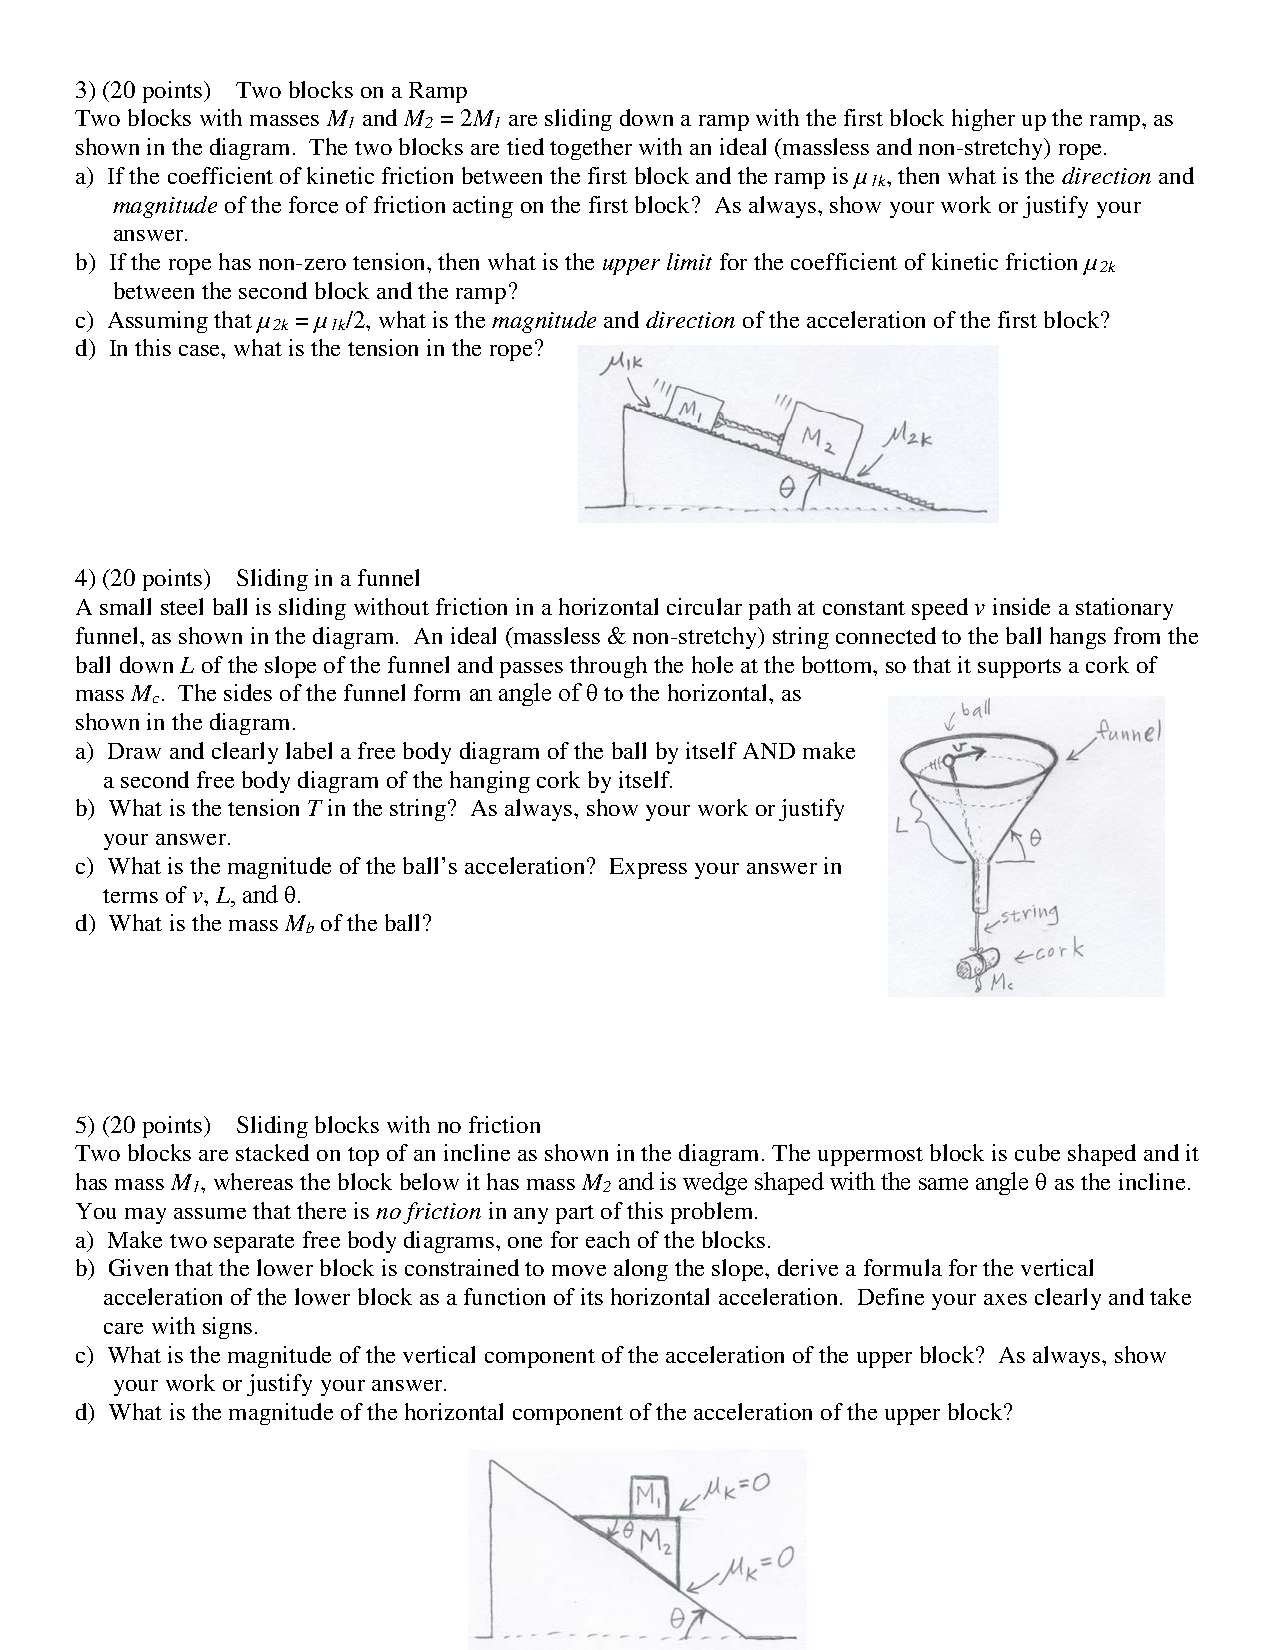
\includepdf[pages=-]{figs/0627/dewese.pdf}
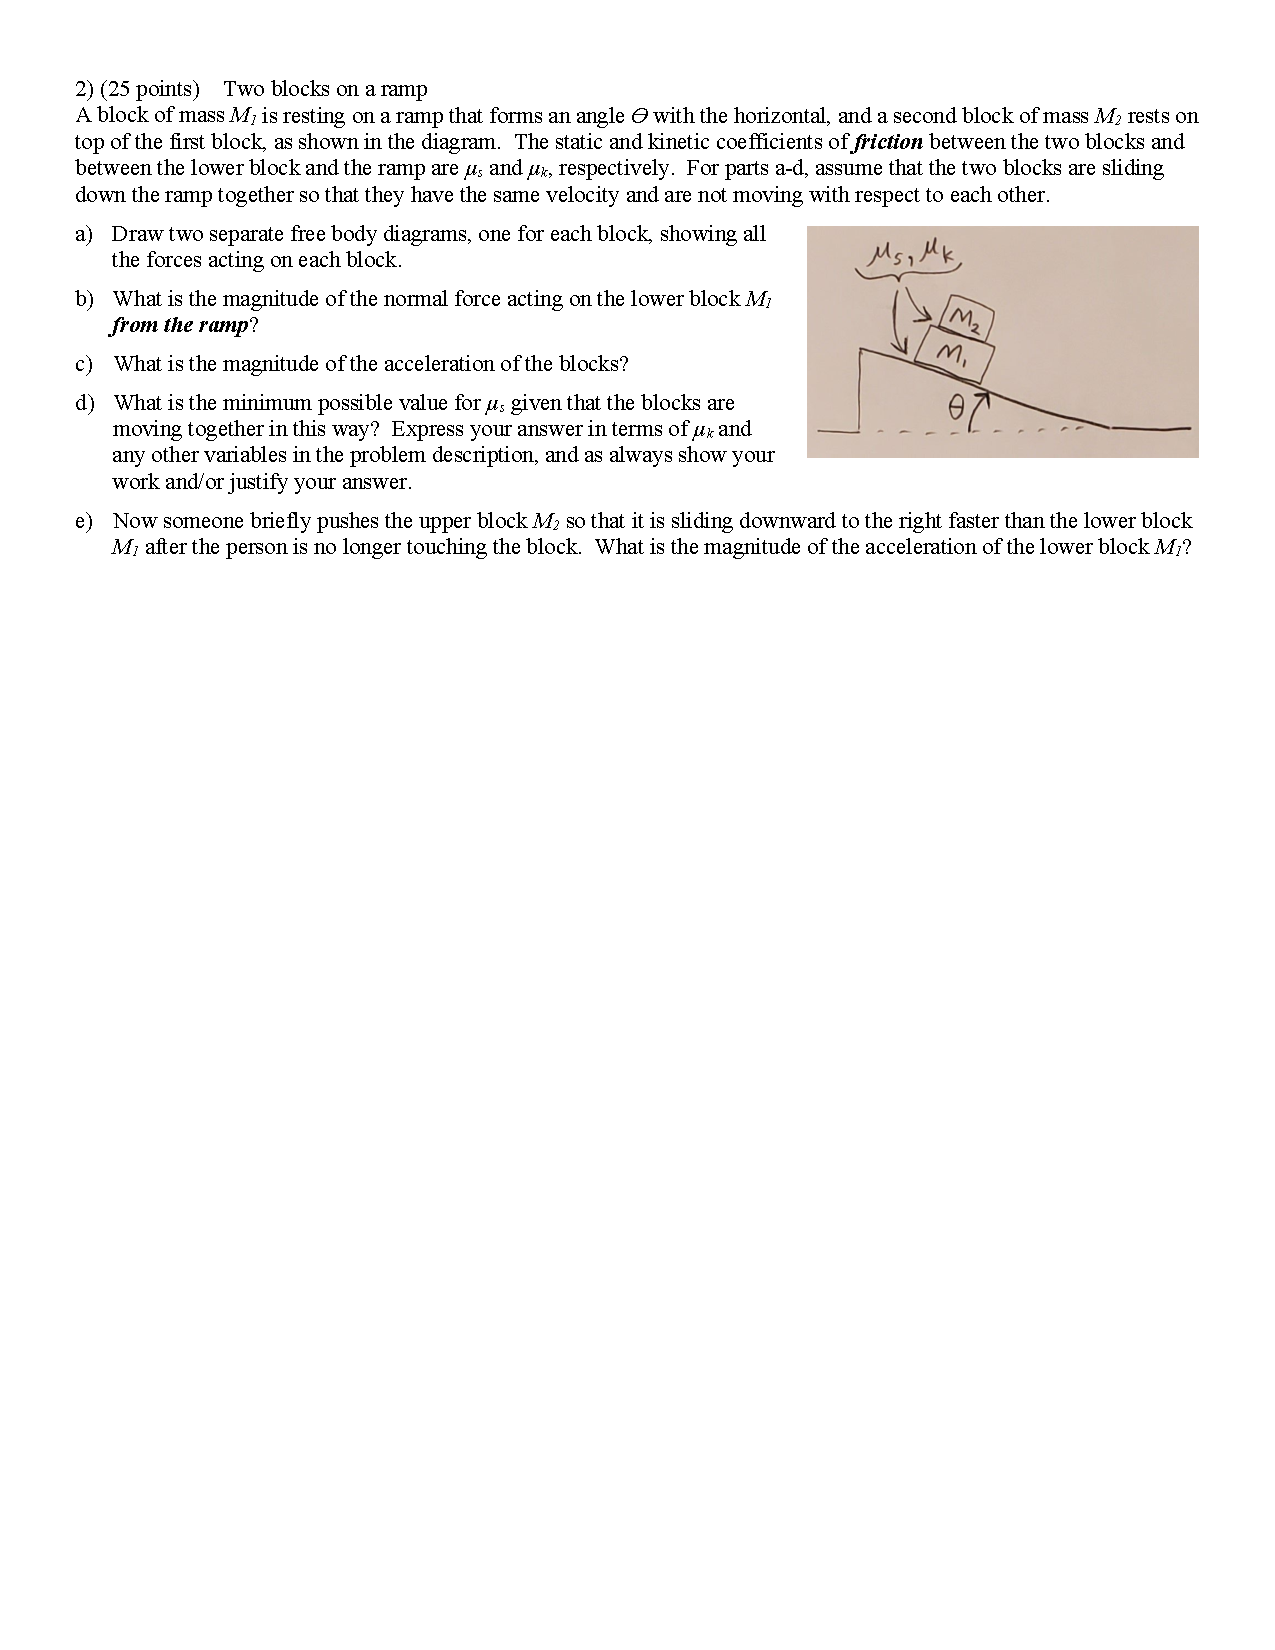
\includepdf[pages=-]{figs/0627/problem_2.pdf}
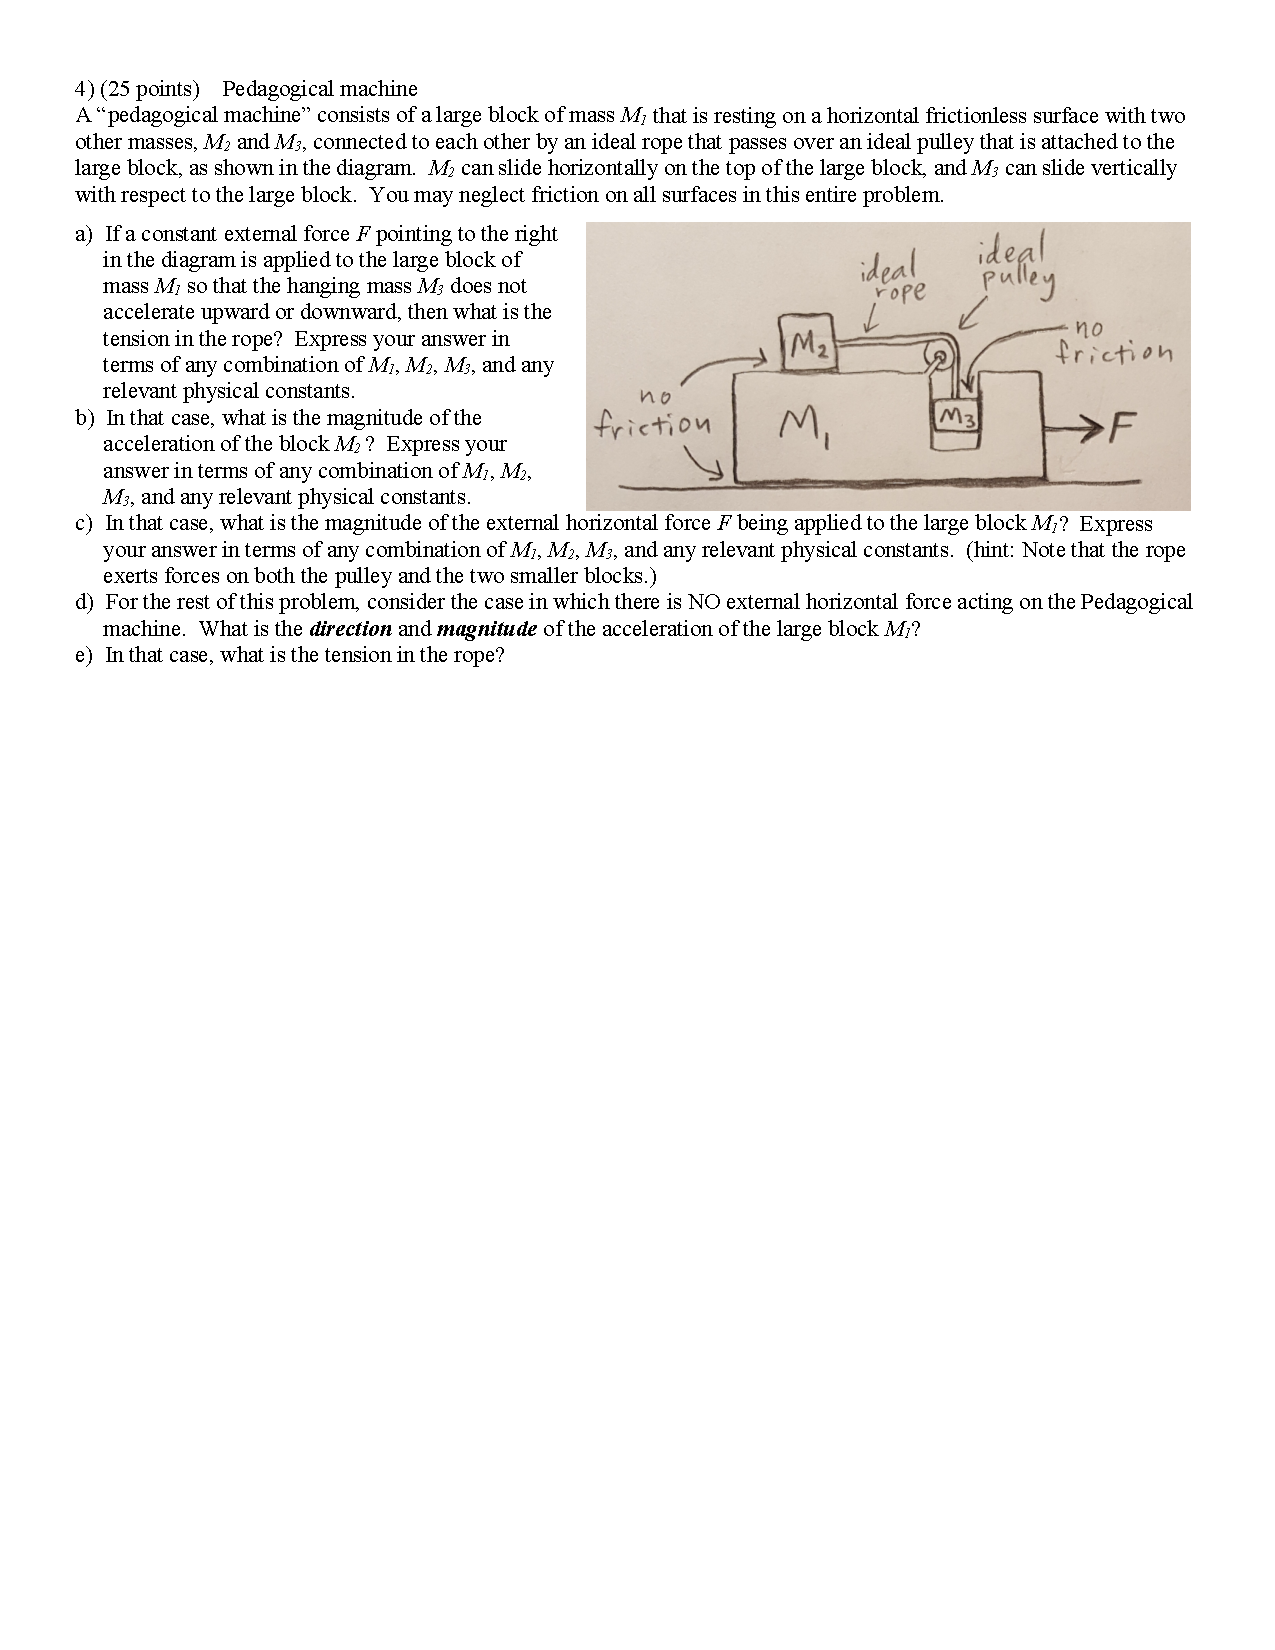
\includepdf[pages=-]{figs/0627/problem_4.pdf}

\end{document}
